\documentclass{article}

\usepackage[utf8]{inputenc}
\usepackage{geometry}
\usepackage{listings}
\usepackage{graphicx}
\usepackage{geometry}
\usepackage{courier}
\usepackage{hyperref}
\usepackage{animate}
\usepackage{amsmath}


%\graphicspath{{../images/}}

\title{HW 8 \\ Game of Life}
\author{Philip Nelson}
\date{2018 October 26}

\lstset{basicstyle=\footnotesize\ttfamily\normalsize,
        breaklines=true,
        stepnumber=1,
       }

\begin{document}

\maketitle

\section*{Introduction}

The purpose of this assignment is to simulate Conway's Game of Life taking advantage of parallelization through MPI. The program begins by populating the world such that there is a one in five chance of a cell being alive. Then it splits the world up groups of rows and sends them to the other processes. Each process then exchanges information with the processes to the ``north'' $((\text{rank} - 1) + \text{world\_size}) \% \text{world\_size}$ and to the ``south'' $(\text{rank} + 1) \% \text{world\_size}$. They each determine the state of their strip for the next generation and send the results to the master to be displayed or saved as pngs. This is repeated until the maximum number of generations is reached. The world can be displayed in ascii on the terminal, or saved as a png and combined into an animated gif. The command line arguments are the world width, world height, number of generations to simulate whether or not to output and output type (0 - ascii, 1 - png/gif).

\section*{Code}
The code is broken up into seven files, main.cpp, communication.hpp, rules.hpp, cell.hpp, random.hpp, output.hpp, and writePNG.hpp. The files are included below.

\bigskip

\subsection{main.cpp}
\lstinputlisting[showstringspaces=false, language=c++, numbers=left]{../main.cpp}

\subsection{communication.hpp}
\lstinputlisting[showstringspaces=false, language=c++, numbers=left]{../communication.hpp}

\subsection{rules.hpp}
\lstinputlisting[showstringspaces=false, language=c++, numbers=left]{../rules.hpp}

\subsection{cell.hpp}
\lstinputlisting[showstringspaces=false, language=c++, numbers=left]{../cell.hpp}

\subsection{random.hpp}
\lstinputlisting[showstringspaces=false, language=c++, numbers=left]{../random.hpp}

\subsection{output.hpp}
\lstinputlisting[showstringspaces=false, language=c++, numbers=left]{../output.hpp}

\subsection{writePNG.hpp}
\lstinputlisting[showstringspaces=false, language=c++, numbers=left]{../writePNG.hpp}
\newpage

\section*{Output}

\begin{lstlisting}[showstringspaces=false]

# mpic++ -O3 -lpng main.cpp -o gameOfLife.out

# mpiexec --oversubscribe -n 5 gameOfLife.out 1024 1024 25 0 0

Simulating:
---------------------

1020 x 1020 world
Processes: 5
Rows Per Process: 204
Make output: false
---------------------

Simulation Time: 0.243867
Image Write Time: 5.0079e-06
gif Creating time: 5.90226e-08

# mpiexec --oversubscribe -n 5 gameOfLife.out 10 10 10 1 0

Simulating:
---------------------

10 x 10 world
Processes: 5
Rows Per Process: 2
Make output: true
---------------------

..........
.....*....
........*.
*.*....*..
........*.
.......*..
.......**.
..........
.....**...
....*.....
----------
..........
..........
..........
.......**.
.......**.
.......*..
.......**.
......**..
.....*....
.....*....
----------
generation 0 complete
..........
..........
..........
.......**.
......*...
......*...
........*.
......***.
.....*....
..........
----------
generation 1 complete
..........
..........
..........
.......*..
......*...
.......*..
......*.*.
......***.
......**..
..........
----------
generation 2 complete
..........
..........
..........
..........
......**..
......**..
......*.*.
.....*..*.
......*.*.
..........
----------
generation 3 complete
..........
..........
..........
..........
......**..
.....*..*.
.....**.*.
.....**.**
.......*..
..........
----------
generation 4 complete
..........
..........
..........
..........
......**..
.....*..*.
....*...*.
.....*..**
......***.
..........
----------
generation 5 complete
..........
..........
..........
..........
......**..
.....**.*.
....**.**.
.....**..*
......****
.......*..
----------
generation 6 complete
..........
..........
..........
..........
.....***..
....*...*.
....*...**
....*....*
.....*...*
......**..
----------
generation 7 complete
..........
..........
..........
......*...
.....***..
....*.*.**
...***..**
....**...*
.....**.*.
......*...
----------
generation 8 complete
..........
..........
..........
.....***..
........*.
...*.....*
...*..**..
...*...*.*
....*.**..
.....***..
----------
generation 9 complete

Simulation Time: 0.0599119
Image Write Time: 10.0065
gif Creating time: 0.439408

\end{lstlisting}

\section*{Findings} The findings were fairly unsurprising. My computer has two cores with hyper-threading and it is clear to see that performance improves as the number of processes increases until it surpasses the hardware. The graph below shows a 1024 x 1024 world simulated for 500 generations.

\begin{figure}[!htbp]
    \centering
    \fbox{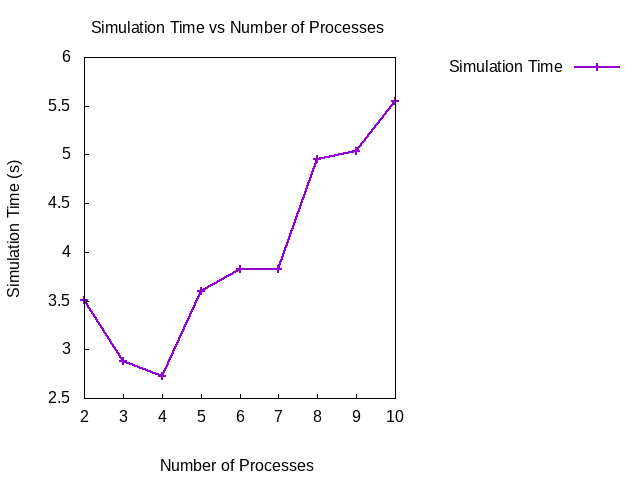
\includegraphics[width=150mm]{./images/benchmark.png}}%tabe size
    \label{fig:graph1}
\end{figure}

\begin{figure}[!htbp]
  \animategraphics[loop,controls,width=\linewidth]{12}{images/}{1}{100}
  \caption{Conway's Game of Life GIF}
\end{figure}

\end{document}
